\documentclass[12pt,a4paper]{extarticle}
\usepackage[utf8]{inputenc}
\usepackage[T5]{fontenc}
\usepackage{geometry}
\geometry{a4paper, left=1.5cm, right=1cm, top=1.5cm, bottom=1.5cm, headheight=20pt, headsep=15pt, footskip=28pt}
\usepackage{enumitem}
\usepackage{amssymb}
\usepackage{setspace}
\usepackage{tikz}
\definecolor{book}{RGB}{58,90,172}
\newcommand{\noteicon}{\textcolor{book}{$\blacktriangleright$}}
\usetikzlibrary{patterns, patterns.meta, calc} % Thêm patterns.meta vào đây
% Gọi package nằm trong thư mục con template
\usepackage{../template/mngocbox}

\begin{document}
\onehalfspacing

% Sử dụng ngoặc vuông [...] để thay đổi linh hoạt các thông số
\makeheadbox[headerright={Tổng ôn 10-11},chude={CHỦ ĐỀ 04},tieude={Oxy, ba đường conic},dinhdang={Hình học},lop={12 },gv={Nguyễn Lê Minh Ngọc}]

\vspace{2em}
\makeheading{IV}{Bài tập thực hành}
\textbf{Câu 1.} Một người đang viết chương trình cho trò chơi bóng đá rô bốt. Gọi $A(-1; 1), B(9; 6), C(5; -3)$ là ba vị trí trên màn hình.\\
\begin{center}
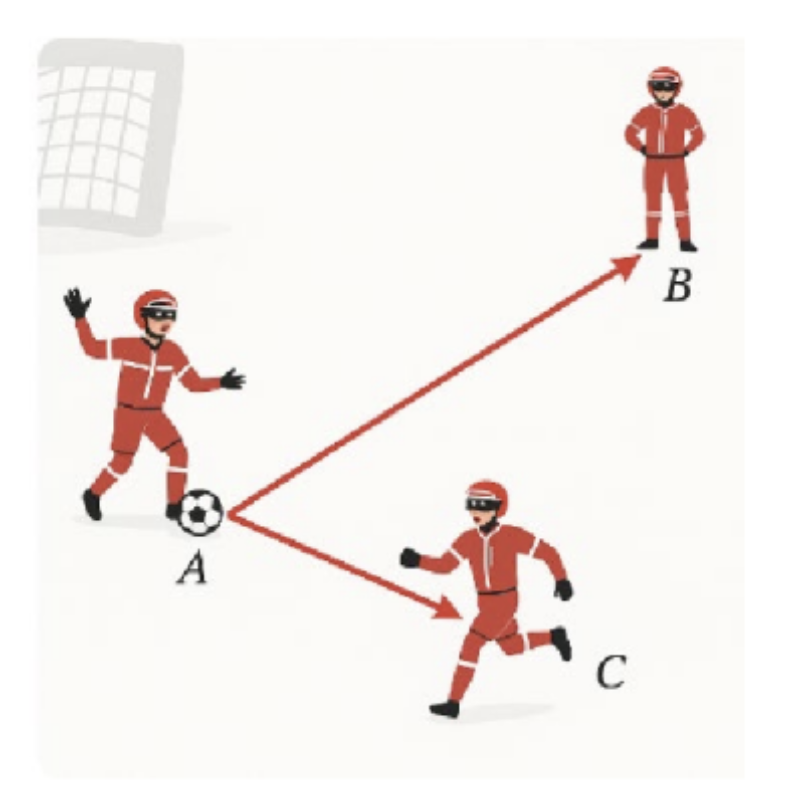
\includegraphics[width=0.3\textwidth]{5.11.png}
\end{center}
a) Viết phương trình các đường thẳng $AB, AC, BC$.\\

b) Tính góc hợp bởi hai đường thẳng $AB$ và $AC$.\\

c) Tính khoảng cách từ điểm $A$ đến đường thẳng $BC$.\\

\textbf{Câu 2.} Động đất hay địa chấn là sự rung chuyển trên bề mặt Trái Đất do kết quả của sự giải phóng năng lượng bất ngờ ở lớp vỏ Trái Đất và phát sinh ra sóng địa chấn (\textit{theo Wikipedia}) với mô hình động đất được cho như hình bên. Ngày 06/02/2023, một trận động đất cường độ 7,8 độ richter có tâm chấn tại Thổ Nhĩ Kì được mô tả bởi tâm $I$ của đường tròn tác động $(C)$ trong mặt phẳng tọa độ $Oxy$ (đơn vị trên hai trục tọa độ là ki-lô-mét). Biết rằng đường tròn tác động $(C)$ đi qua hai thành phố Kahramamaras và Nurdagi được mô tả bởi hai điểm $K(-3; 10)$ và $N(8; 0)$; tâm chấn $I$ có hoành độ dương và cách thành phố Aleppo của Syria được mô tả bởi điểm $G\left(9; \dfrac{-17}{4}\right)$ là $4\sqrt{10} km$. Tìm bán kính ($km$) của đường tròn $(C)$ (kết quả làm tròn đến hàng phần trăm).\\
\begin{center}
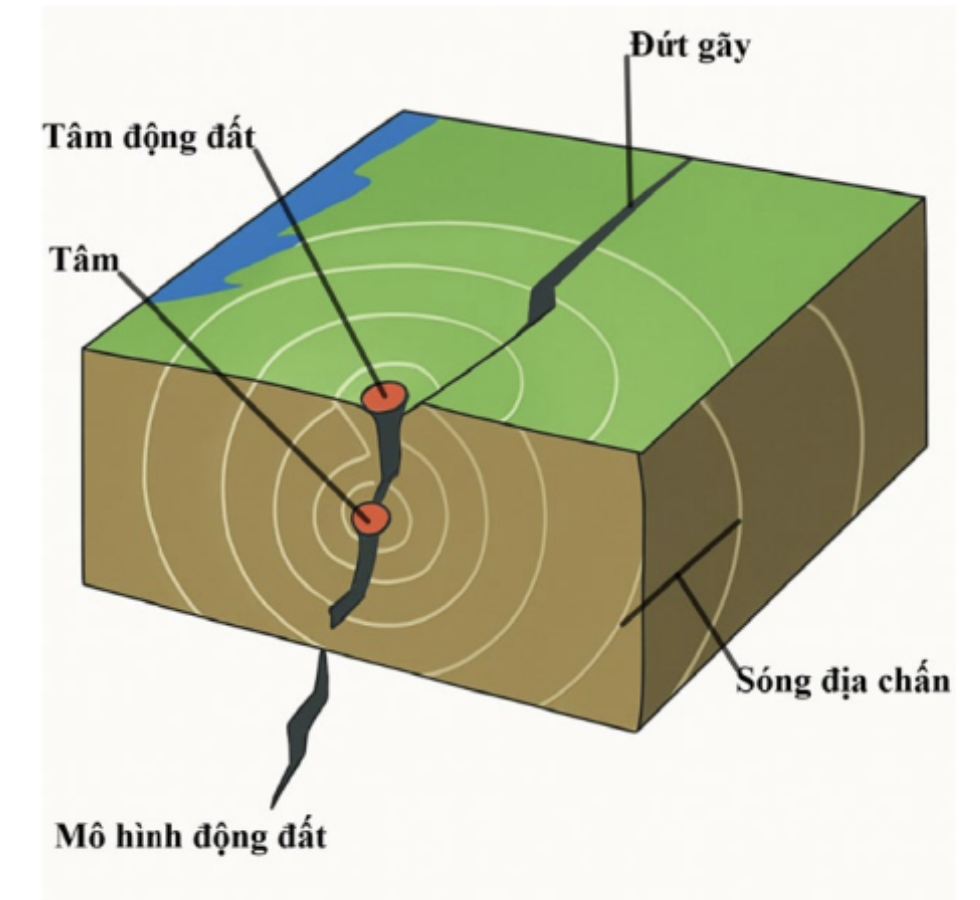
\includegraphics[width=0.3\textwidth]{5.12.png}
\end{center}
Nguồn ảnh: Tìm hiểu về nguyên nhân gây động đất\\

$\Rightarrow$ Đáp số: ..........

\textbf{Câu 3.} Một nông trại tưới nước theo phương pháp vòi phun xoay vòng trung tâm như hình bên. Cho biết tâm một vòi phun được đặt tại tọa độ $(12; -9)$ và vòi có thể phun xa tối đa $36$ m. Hãy viết phương trình đường tròn biểu diễn tập hợp các điểm xa nhất mà vòi nước có thể phun tới.\\
\begin{center}
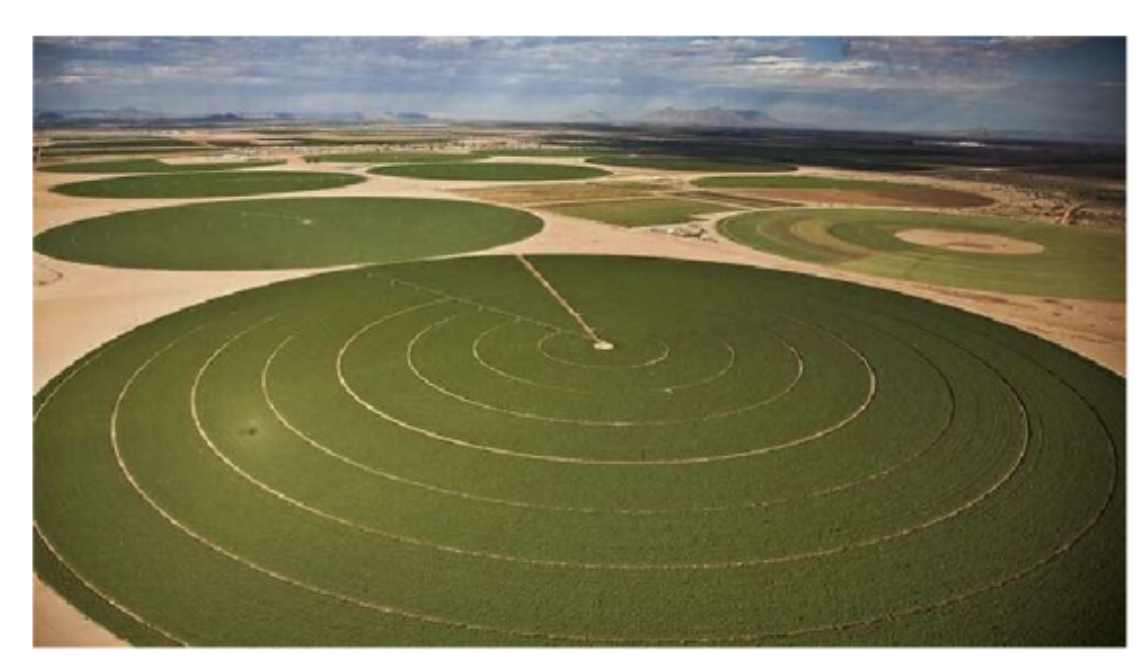
\includegraphics[width=0.3\textwidth]{5.13.png}
\end{center}
$\Rightarrow$ Đáp số: ..........\\
\vspace{0.5cm}
\textbf{Câu 4.} Một nhà vòm chứa máy bay có mặt cắt hình nửa elip cao $10$ m, rộng $24$ m.\\
\begin{center}
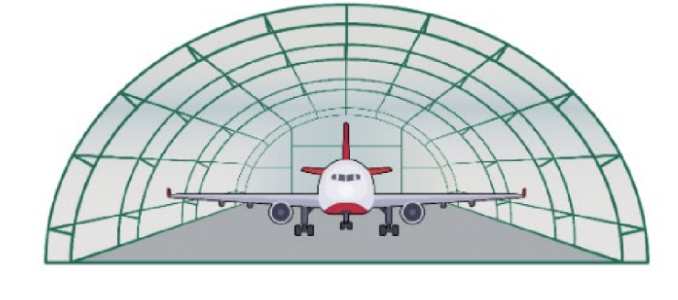
\includegraphics[width=0.3\textwidth]{6.6.png}
\end{center}
a) Chọn hệ tọa độ thích hợp và viết phương trình của elip nói trên.

b) Tính khoảng cách theo phương thẳng đứng từ một điểm cách chân tường $4$ m lên đến nóc nhà vòm.

$\Rightarrow$ Đáp số: ..........

\textbf{Câu 5.} Vệ tinh nhân tạo đầu tiên được Liên Xô (cũ) phóng từ Trái Đất năm 1957. Quỹ đạo của vệ tinh đó là một đường elip nhận tâm Trái Đất là một tiêu điểm có phương trình quỹ đạo là $\dfrac{x^2}{a^2} + \dfrac{y^2}{b^2} = 1$. Người ta đo được vệ tinh cách bề mặt Trái Đất gần nhất là $583$ dặm và xa nhất là $1342$ dặm ($1$ dặm xấp xỉ $1,609$ km). Tìm tỷ số $\dfrac{c}{a}$, biết bán kính của Trái Đất xấp xỉ $4000$ dặm.
\begin{center}
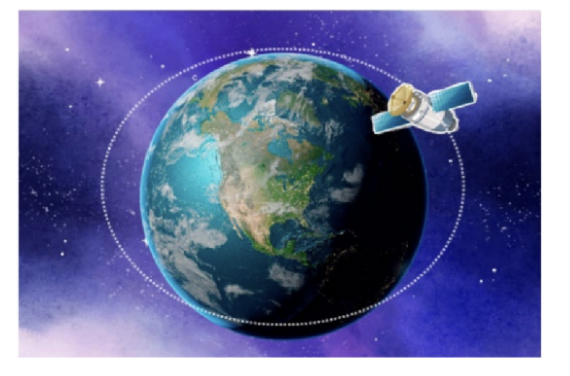
\includegraphics[width=0.3\textwidth]{6.7.png}
\end{center}
$\Rightarrow$ Đáp số: ..........

\textbf{Câu 6.} Một tháp làm nguội của một nhà máy có mặt cắt là hình hypebol có phương trình $\dfrac{x^2}{64^2} - \dfrac{y^2}{35^2} = 1$. Biết chiều cao của tháp là $210$ m và khoảng cách từ nóc tháp đến tâm đối xứng của hypebol bằng một nửa khoảng cách từ tâm đối xứng tới đáy. Tính bán kính đáy của tháp. (Làm tròn đến hàng đơn vị)
\begin{center}
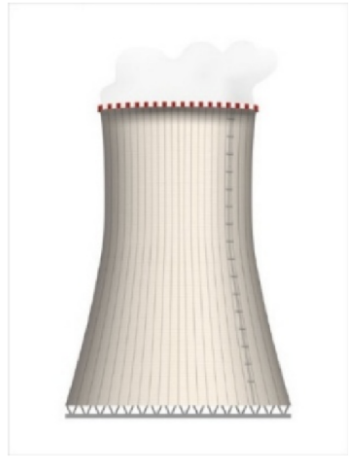
\includegraphics[width=0.3\textwidth]{6.8.png}
\end{center}
$\Rightarrow$ Đáp số: ..........
\end{document}